\documentclass{beamer}

\usepackage[utf8]{inputenc} % Включаем поддержку UTF8  
\usepackage[russian]{babel} % Включаем пакет для поддержки русского языка 

\title[Spherical Principal Component Analysis]{Spherical Principal Component Analysis}

\subtitle{Applying spherical PCA algorithm for dimensionality reduction set of unit vectors}

\author[] { Белоусов Илларион, Карчмит Илья, Курбет Игорь, Малашенко Сергей, Машинсон Всеволод, Свиридов Илья, Панов Алексей }

\date[]{OZON Masters, December 2020}

\begin{document}

\frame{\titlepage}

\begin{frame}
\frametitle{Постановка задачи}
\begin{itemize}
 \item В задачах классификации и распознавания объектов хорошо себе зарекомендовали модели, которые оценивают близость 
 $$X_i \in S^n = \{ x \in \mathbb{R}^{n+1} : \left\lVert x \right\rVert=1 \}$$
 \item В процессе разработки модели размерность пространства $n$ может быть достаточно большой, что приводит к трудностям в использовании модели.
 \item В работе предлагается снизить размерность $n$ при помощи метода $SphericalPCA$, который позволит от $S^n \Rightarrow S^m$, где $m < n$.
 \item Качество алгоритма оценивается решением задачи кластеризации векторов $X_i \in S^n, \tilde{X_i} \in S^m$ в предположении, что $$X_i \sim \sum_{i=1}^{N}\pi_i \mathbb{V}_{n+1}(x | \mu_i, \kappa_i), \mathbb{V}(x | \mu_i, \kappa_i)=C_{n+1}(\kappa) e^{\kappa \mu^{\top} x}$$
\end{itemize}
\end{frame}

\begin{frame}
\frametitle{Решение задачи}
Решение общей задачи разбивается на три подзадачи
\begin{itemize}
 \item Разработка и сравнение моделей классификации на наборе данных MNIST. Модели строятся с использованием $SoftMax + NLL$, и $ArcFace$. Для функции потерь $ArcFace$ результатом работы будет совокупность $$X_i \in S^n = \{ x \in \mathbb{R}^{n+1} : \left\lVert x \right\rVert=1 \}$$
\item Разработка инструмента, который использует алгоритм $SphericalPCA$ и снижает размерность $X_i \in S^n \Rightarrow \tilde{X_i} \in S^m$, где $m < n$
\item Разработка инструмента, который решает задачу кластеризации векторов 
$X_i \in S^n, \tilde{X_i} \in S^m$ 
$$X_i \sim \sum_{i=1}^{N}\pi_i \mathbb{V}_{n+1}(x | \mu_i, \kappa_i), \tilde{X_i} \sim \sum_{i=1}^{N}\pi_i \mathbb{V}_{m+1}(x | \tilde{\mu_i}, \tilde{\kappa_i})$$
\end{itemize}

\end{frame}

\begin{frame}
\frametitle{Модель классификации}
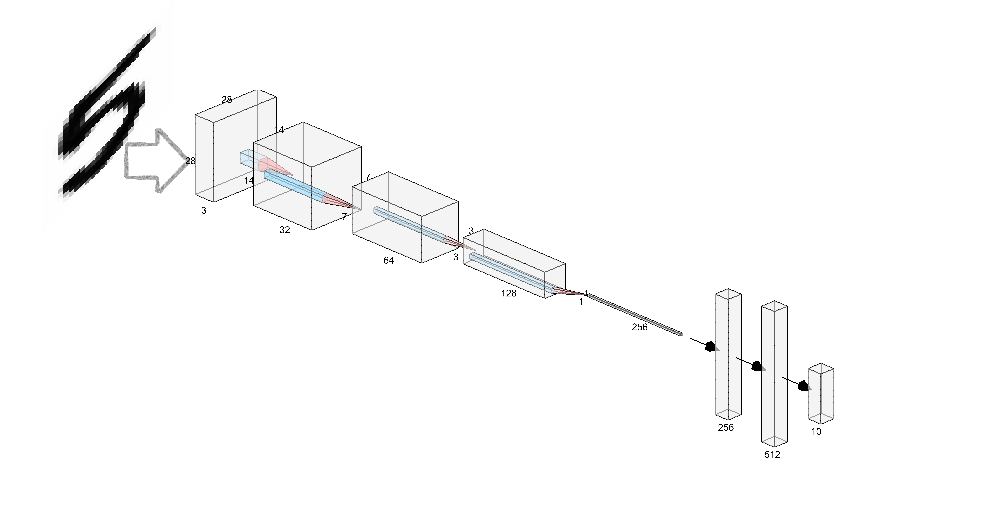
\includegraphics[scale=0.3]{mnist_model.png}
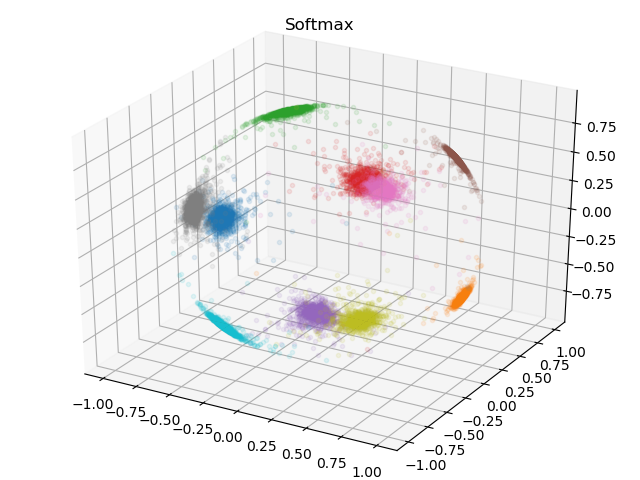
\includegraphics[scale=0.3]{mnist_vgg8_3d.png}
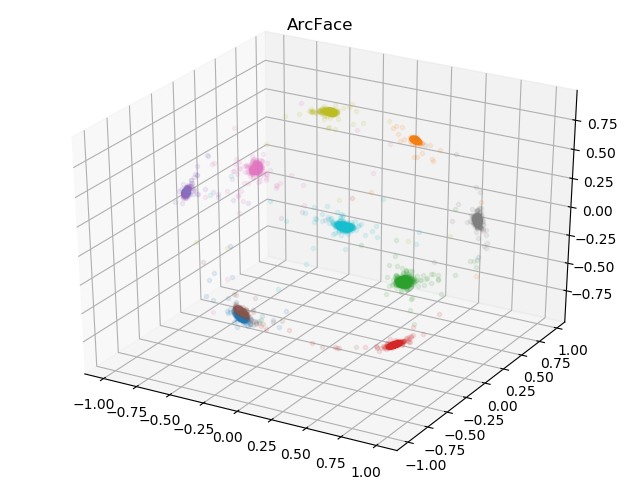
\includegraphics[scale=0.3]{mnist_vgg8_arcface_3d.png}
\end{frame}

\begin{frame}
\frametitle{Алгоритм SphericalPCA}

\end{frame}

\begin{frame}
\frametitle{Кластеризация данных}

\end{frame}

\begin{frame}
\frametitle{Выводы}
\begin{itemize}
\item Использование нормированных векторов в задачах классификации и распознавания, позволяет повысить качество работы модели.
\item Алгоритм SphericalPCA позволяет снизить размерность результирующих векторов, что приводит к повышению локализации кластеров, а также повышению производительности работы общей системы.
\end{itemize}

\end{frame}


\end{document}
